\documentclass[11pt]{article}

\usepackage{amsmath,setspace,mathtools,amssymb,booktabs,graphicx, multicol, bm}

\usepackage[utf8]{inputenc}

\usepackage[letterpaper,portrait,margin=0.5cm]{geometry}

\graphicspath{ {./} }


\title{BPhys450 Final Project}

\author{Thaseus Karkabe-Olson}

\date{}

\begin{document}

	\maketitle

    \raggedright
    
    \section*{Abstract}

           	    	
        For this final project I will focus on creating a preliminary active learning activity with an integrated model that addresses goals 4a and 5. The experiment I conduct will be figuring out how a non-physics person interacts with the model in an effort to identify if I can use the model to teach basic magnetism. I will analyze this by recording observations that I noticed while they completed an activity, and through analyzing their work on the activity that I had them complete.
        
   	    \section*{Program Design}
   	    
   	    	The basic underlying program is relatively simple. It takes an input of charge, velocity, mass, and magnetic field strength and passes it to a dedicated python file. I then needed to solve the following differential equation:
   	    	
   	    	\[m a = q v B\]
   	    	
   	    	I could split this into two equations for the x and y directions
   	    	
   	    	\[m \ddot{x} = q B \dot{y}\]
   	    	
   	    	\[m \ddot{y} = - q B \dot{x}\]
   	    	
   	    	However, Scipy can't solve second order equations, so I had to expand this into four first order equations. I used substitution to get the equations
   	    	
   	    	\[\dot{x} = u\]
   	    	
   	    	\[\dot{u} = q B v\]
   	    	
   	    	\[\dot{y} = v\]
   	    	
   	    	\[\dot{v} = - Q B u\]
   	    	
   	    	and defined a function that contained them. I could then pass an array of initial conditions along with this function to odeint, which is able to numerically solve the differential equations over an array of time. odeint can then spit back out arrays for position and velocity in the x and y directions, which my main file then takes and animates.
   	    	
   	    	The main program is designed to be completely closed (i.e. no access to the python file is necessary) and as intuitive as possible. It's set up like an experiment, with initial values that the user sets up. The program tells the user what the value is for each parameter as they either increase or decrease them. They then have the option to run the experiment once they are satisfied with the parameters they've set up, and can observe the particle's animated motion and trajectory over time. They then have the option to view it again, go back to edit the parameters, or quit.
   	    	
   		\section*{Sample numerical experiments}
   		
   			When the particle has some amount of charge, mass, and velocity and goes through a positive B field, it curves upward in uniform circular motion while the magnetic field is on, as seen here:
   			
   			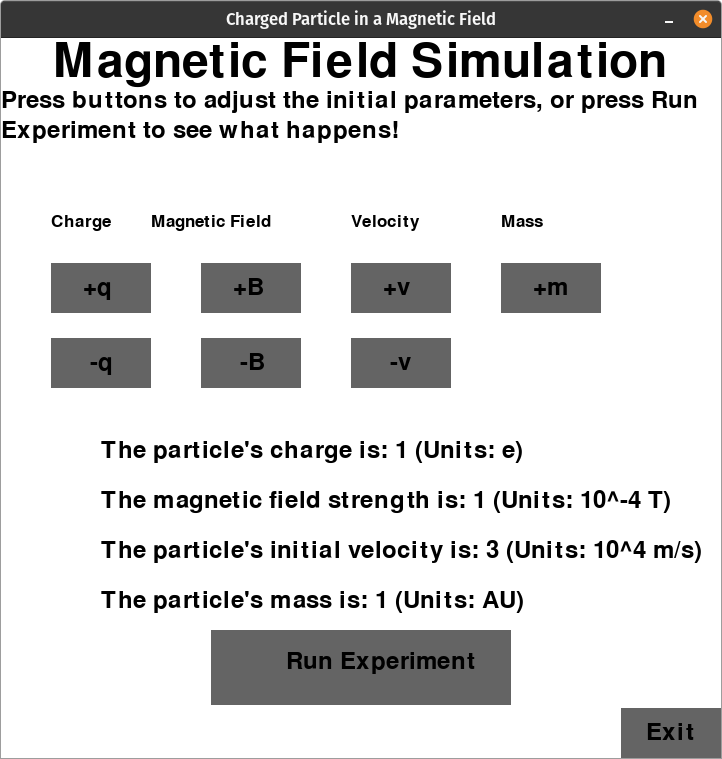
\includegraphics[scale=0.3]{1}
   			
   			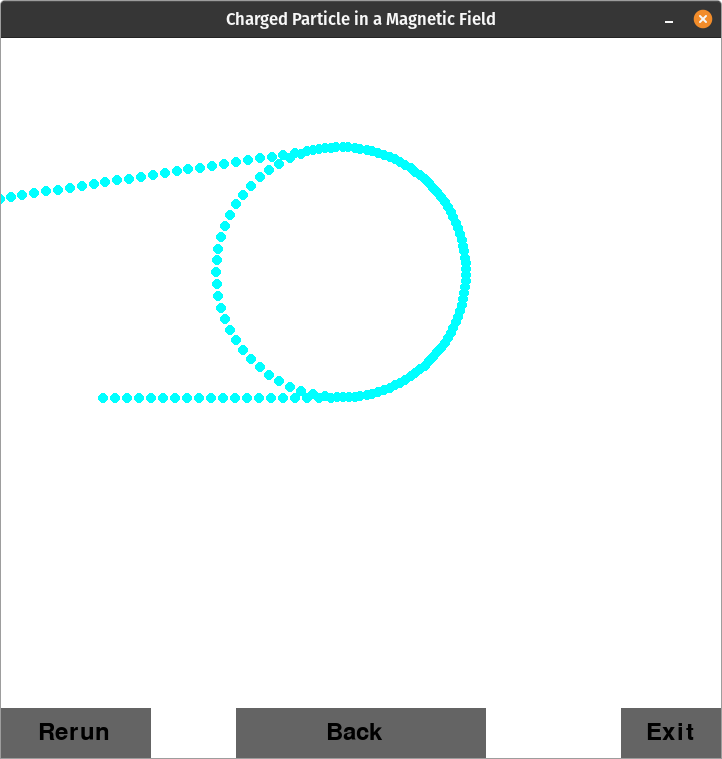
\includegraphics[scale=0.3]{2}
   			
   			If you then increase the charge, your radius of curvature decreases as seen here:
   			
   			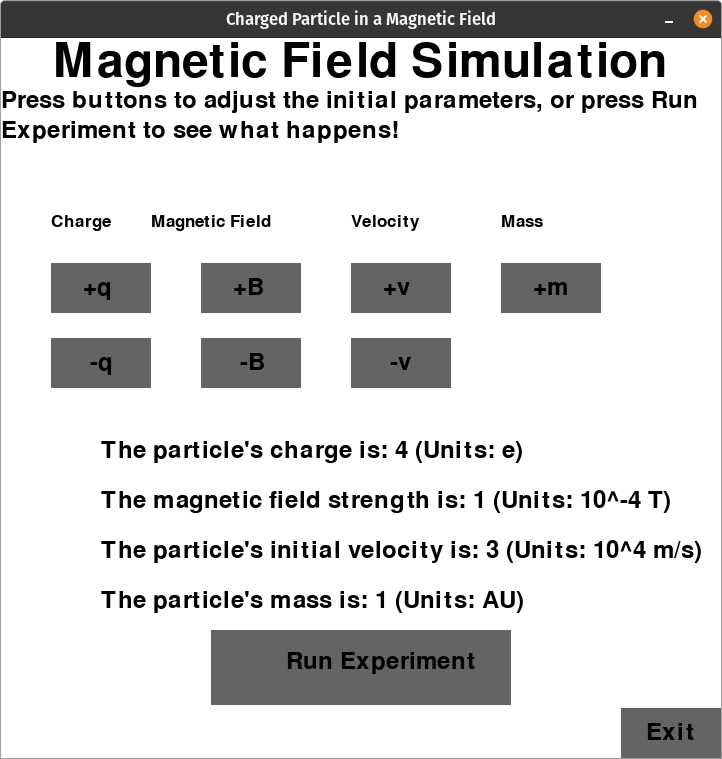
\includegraphics[scale=0.3]{3}
   			
   			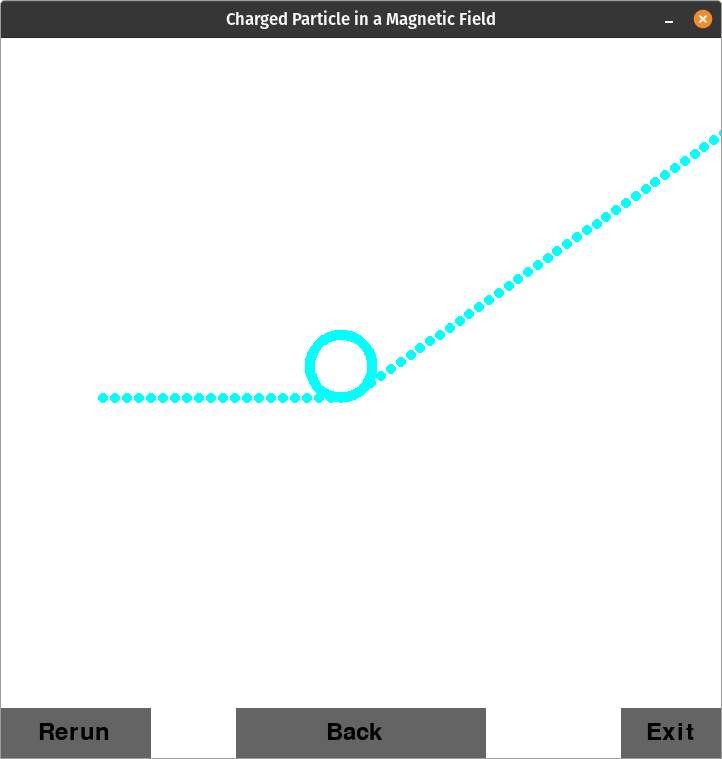
\includegraphics[scale=0.3]{4}
   			
   			If you make the particle negatively charged, the particle deflects the other way, as seen here
   			
   			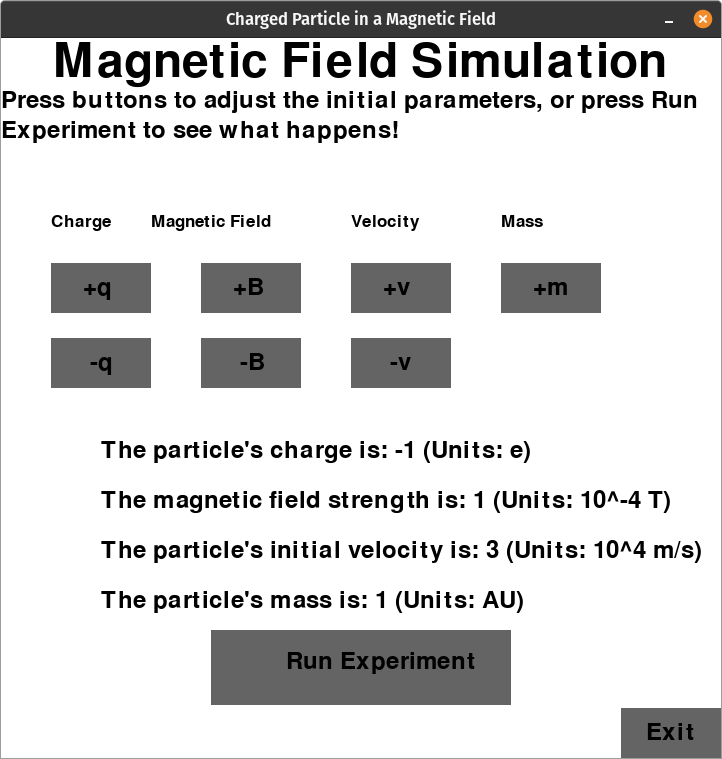
\includegraphics[scale=0.3]{5}
   			
   			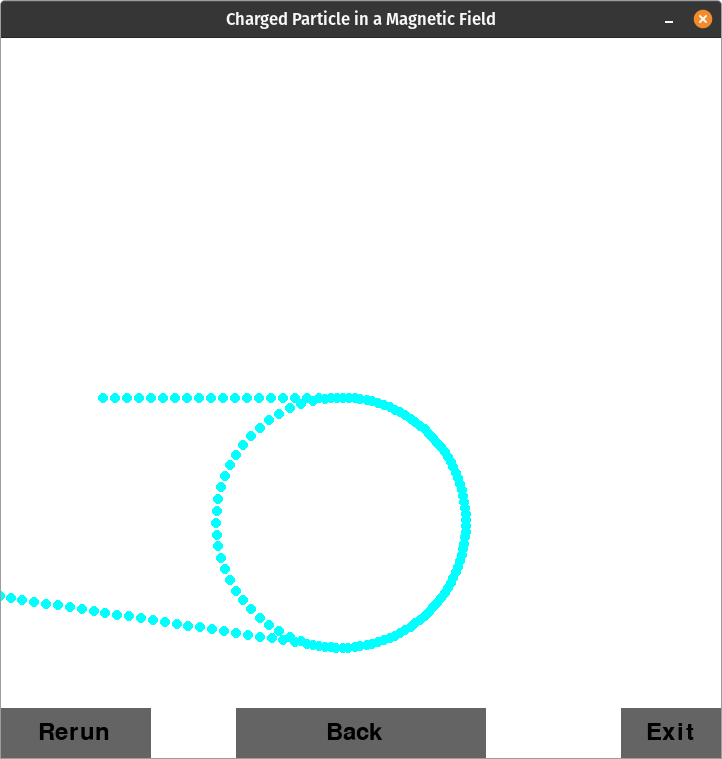
\includegraphics[scale=0.3]{6}
   			
   			And after going through each combination of variables in a similar fashion, you end up seeing the following proportionalities
   			
   			\[r \propto \frac{1}{q},\,\frac{1}{B}\]
   			
   			\[r \propto m,\,v\]
   			
   			Which turn out to directly give you your radius in the following equation
   			
   			\[r = \frac{mv}{qB}\]
   			
   			This is provable using force equations, where
   			
   			\[\frac{m v^2}{r} = q v b\]
   			
   			\[r = \frac{mv}{qB}\]
   			
   			And means that through this experiment a student has the capacity to derive how magnetic force magnitude works, along with understanding the circular motion of a particle
   			
   	    \section*{Problem}
   	    
   	    	The main problem that I aimed to address with this model is the pre-class learning of material and general physics concepts. The goal of this computational model is to enhance student understanding in a preclass activity for a given week. As such, it should be tailored to the learning goals of previous preclass activities. Using the current list of learning goals for week 7 magnatism in BPHYS122 as a reference, students should be able to:
   	    	
   	    	\begin{itemize}
   	    		
   	    		\item Describe similarities and differences between electric and magnetic fields
   	    		\item Use a compass to identify the direction and relative magnitude of a magnetic field, and to identify the north pole of a bar magnet
   	    		\item Draw and interpret magnetic field vectors and field lines: (1) in general, (2) for a bar magnet, (3) for a straight current-carrying wire, and (4) for a loop of current
   	    		\item Calculate the magnetic force on (1) a charged particle moving in a magnetic field, and (2) on a current-carrying wire in a magnetic field
   	    		\item Explain how a charged particle in an external magnetic field undergoes circular motion, and find the radius of that motion
   	    		\item Calculate the force on a current-carrying wire in an external magnetic field (magnitude and direction)
   	    		\item Evaluate the net force on a current loop in an external magnetic field
   	    		\item Evaluate the net torque on a current loop in an external magnetic field
   	    		\item Define the magnetic dipole moment of a current loop
   	    		
   	    	\end{itemize}

   	    	Where the model I used in this case was tailored to goals 4a and 5. Normally, students would learn these principles strictly through reading, so I wanted to enhance their understanding through the development of this model.
   	    	
   	    \section*{Activity}
   	    
   	    My main experiment was designed around goals 4a and 5 and aimed to see how someone without a physics background interacted with the model I designed. As this is focused (at the moment) on qualitative understanding, the questions I present will for the most part be pretty open ended. Here is the activity that I designed:
   	    
   	    \subsection*{Introduction}
   	    
   	    	In this activity you will interact with a model. This model involves a particle with mass, velocity, and charge. When the experiment is run, the particle will travel through empty space for some time. Then a magnetic field pointing either into the page (marked with Xs) or out of the page (marked with dots) will appear for some time. Then the field will turn off.
   	    
   	    \subsection*{Question 1}
			Change some parameters and run some experiments. Write down 5 observations that you noticed.
			
		\subsection*{Question 2}
			\subsubsection*{Part a}
				What are some ways that you can get the particle to travel in a straight line?
				
			\subsubsection*{Part b}
				For each method you listed, why do you think the particle traveled in a straight line?
			
		\subsection*{Question 3}
			Sometimes the particle travels along a curve. How can you relate each of the properties given by the model to the radius of that curve?
			
		\subsection*{Question 4}
			What are two questions you have about the system? \\[12pt]
			
		I then provided this activity and simulation to a family member with no physics background and observed them. Here are their responses:
		
		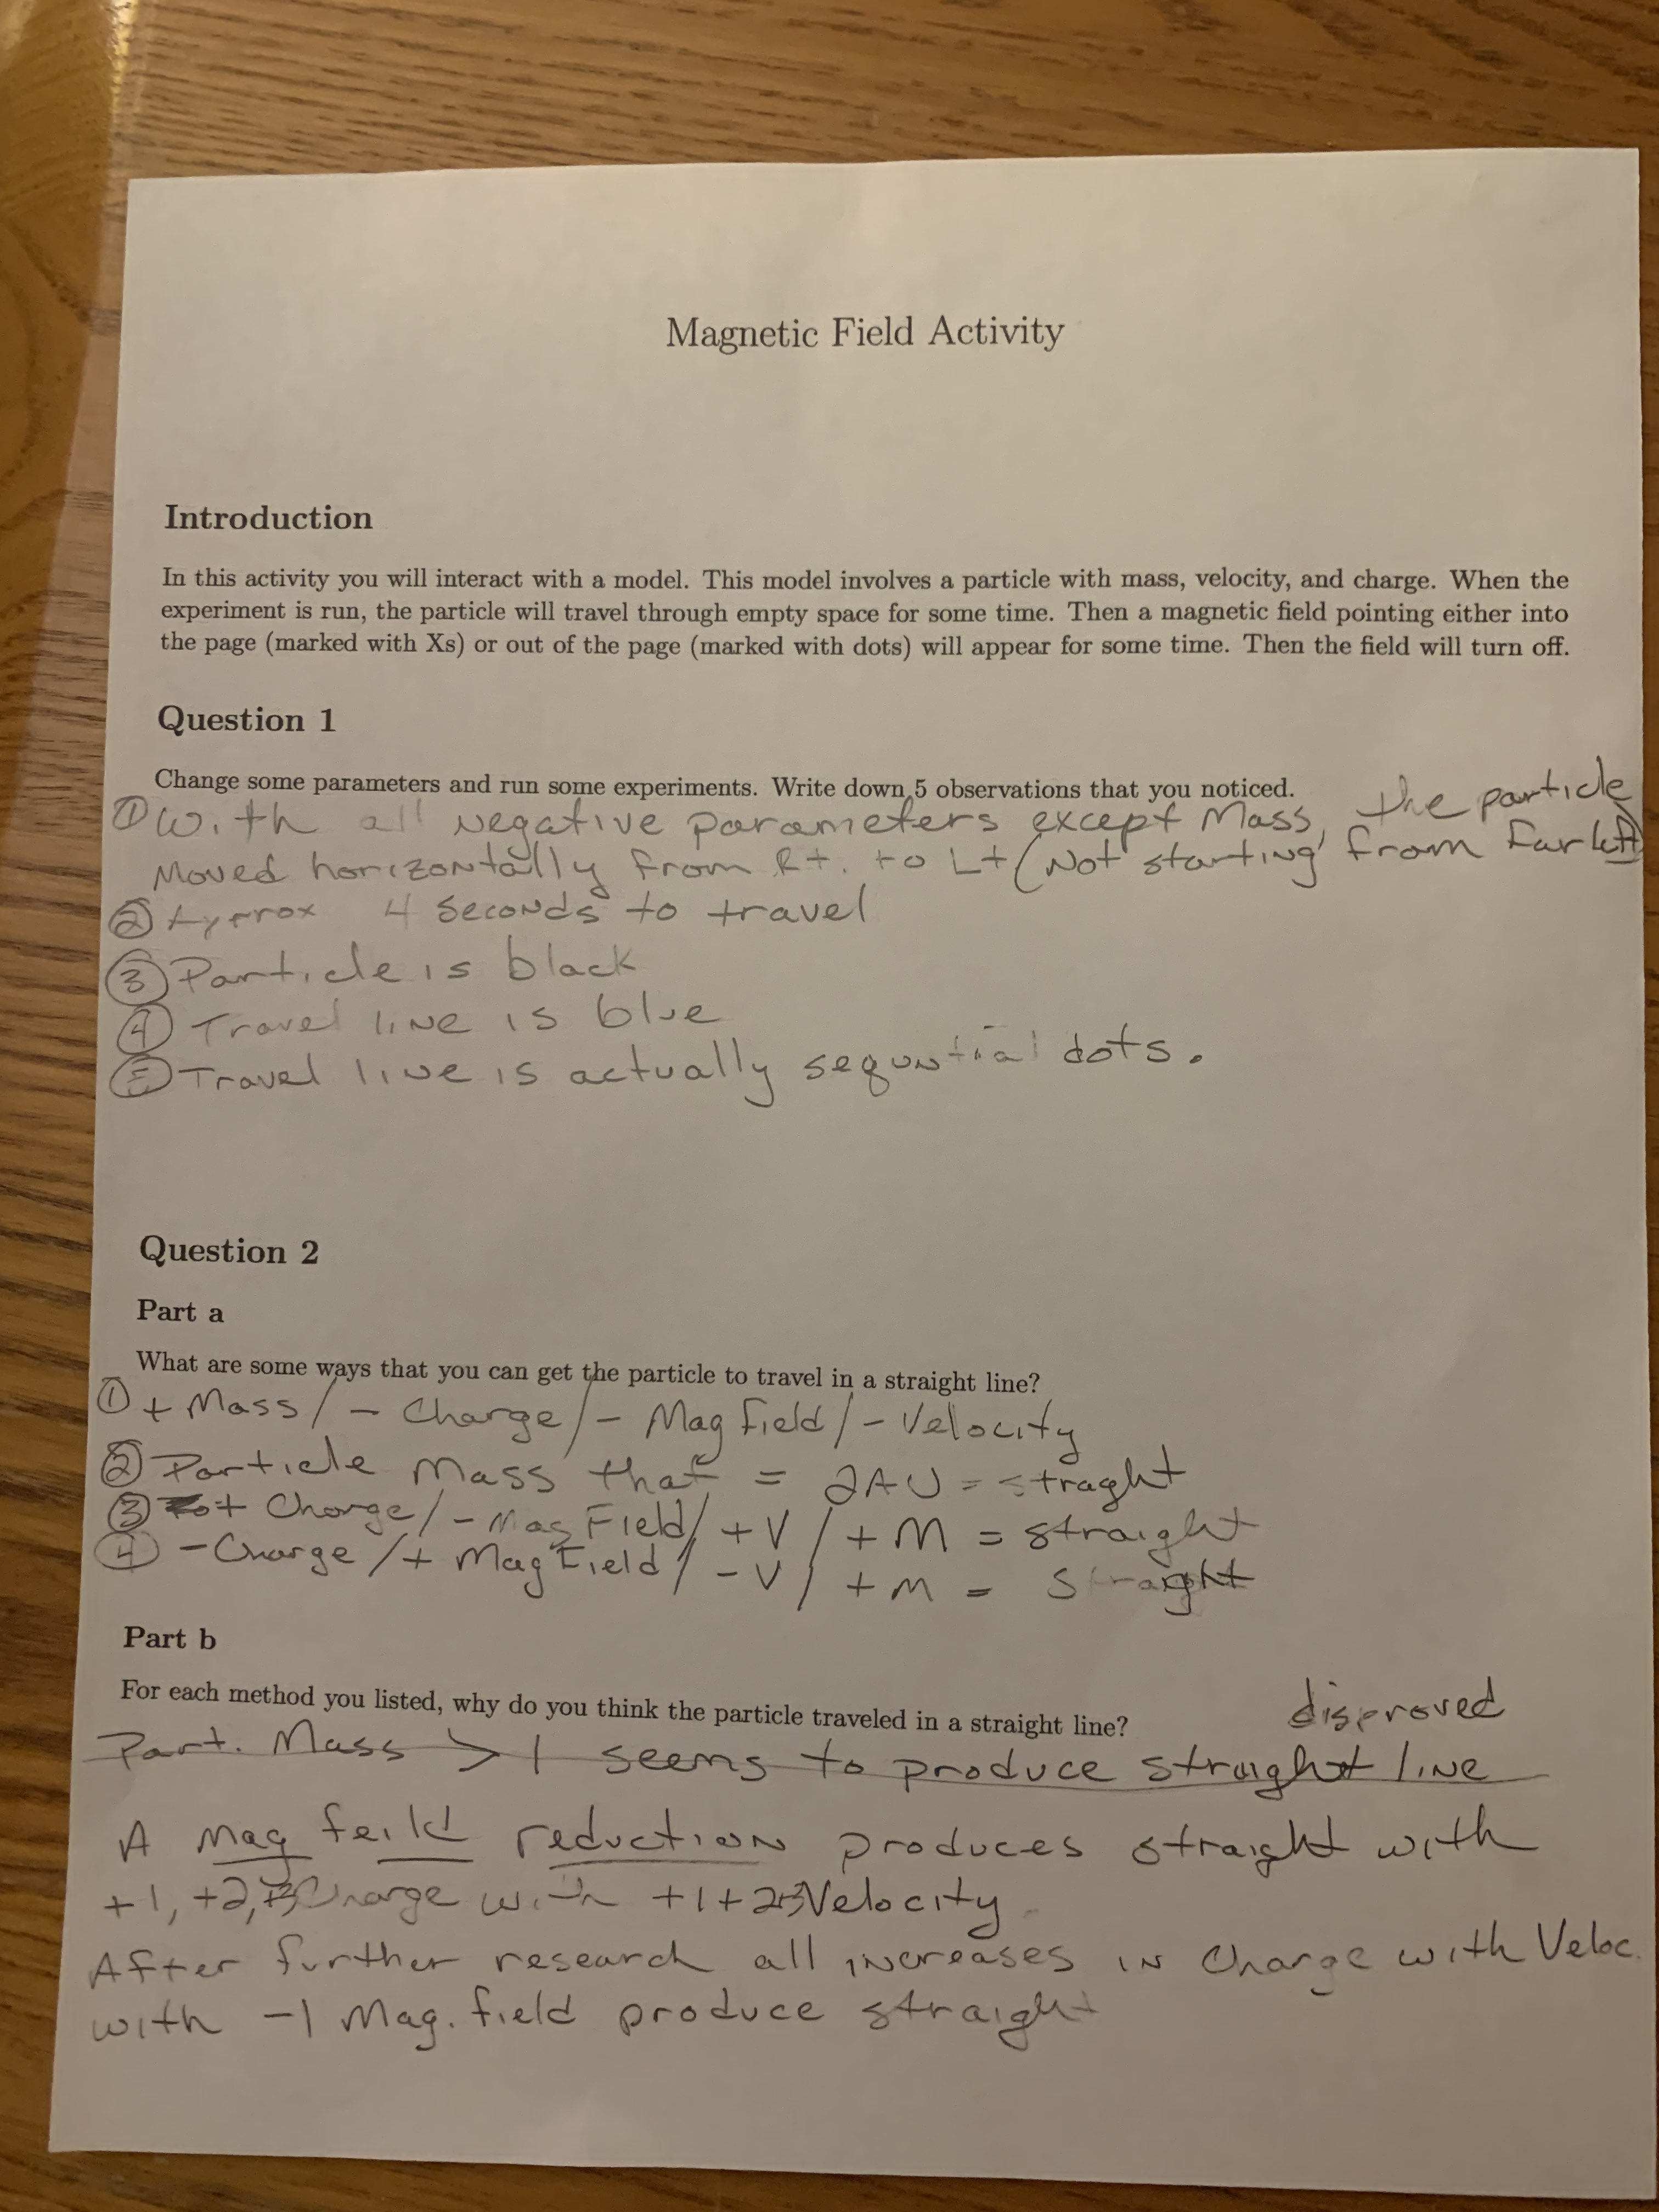
\includegraphics[scale = 0.15]{IMG_1}
		
		
\includegraphics[scale = 0.15]{IMG_2}
		
		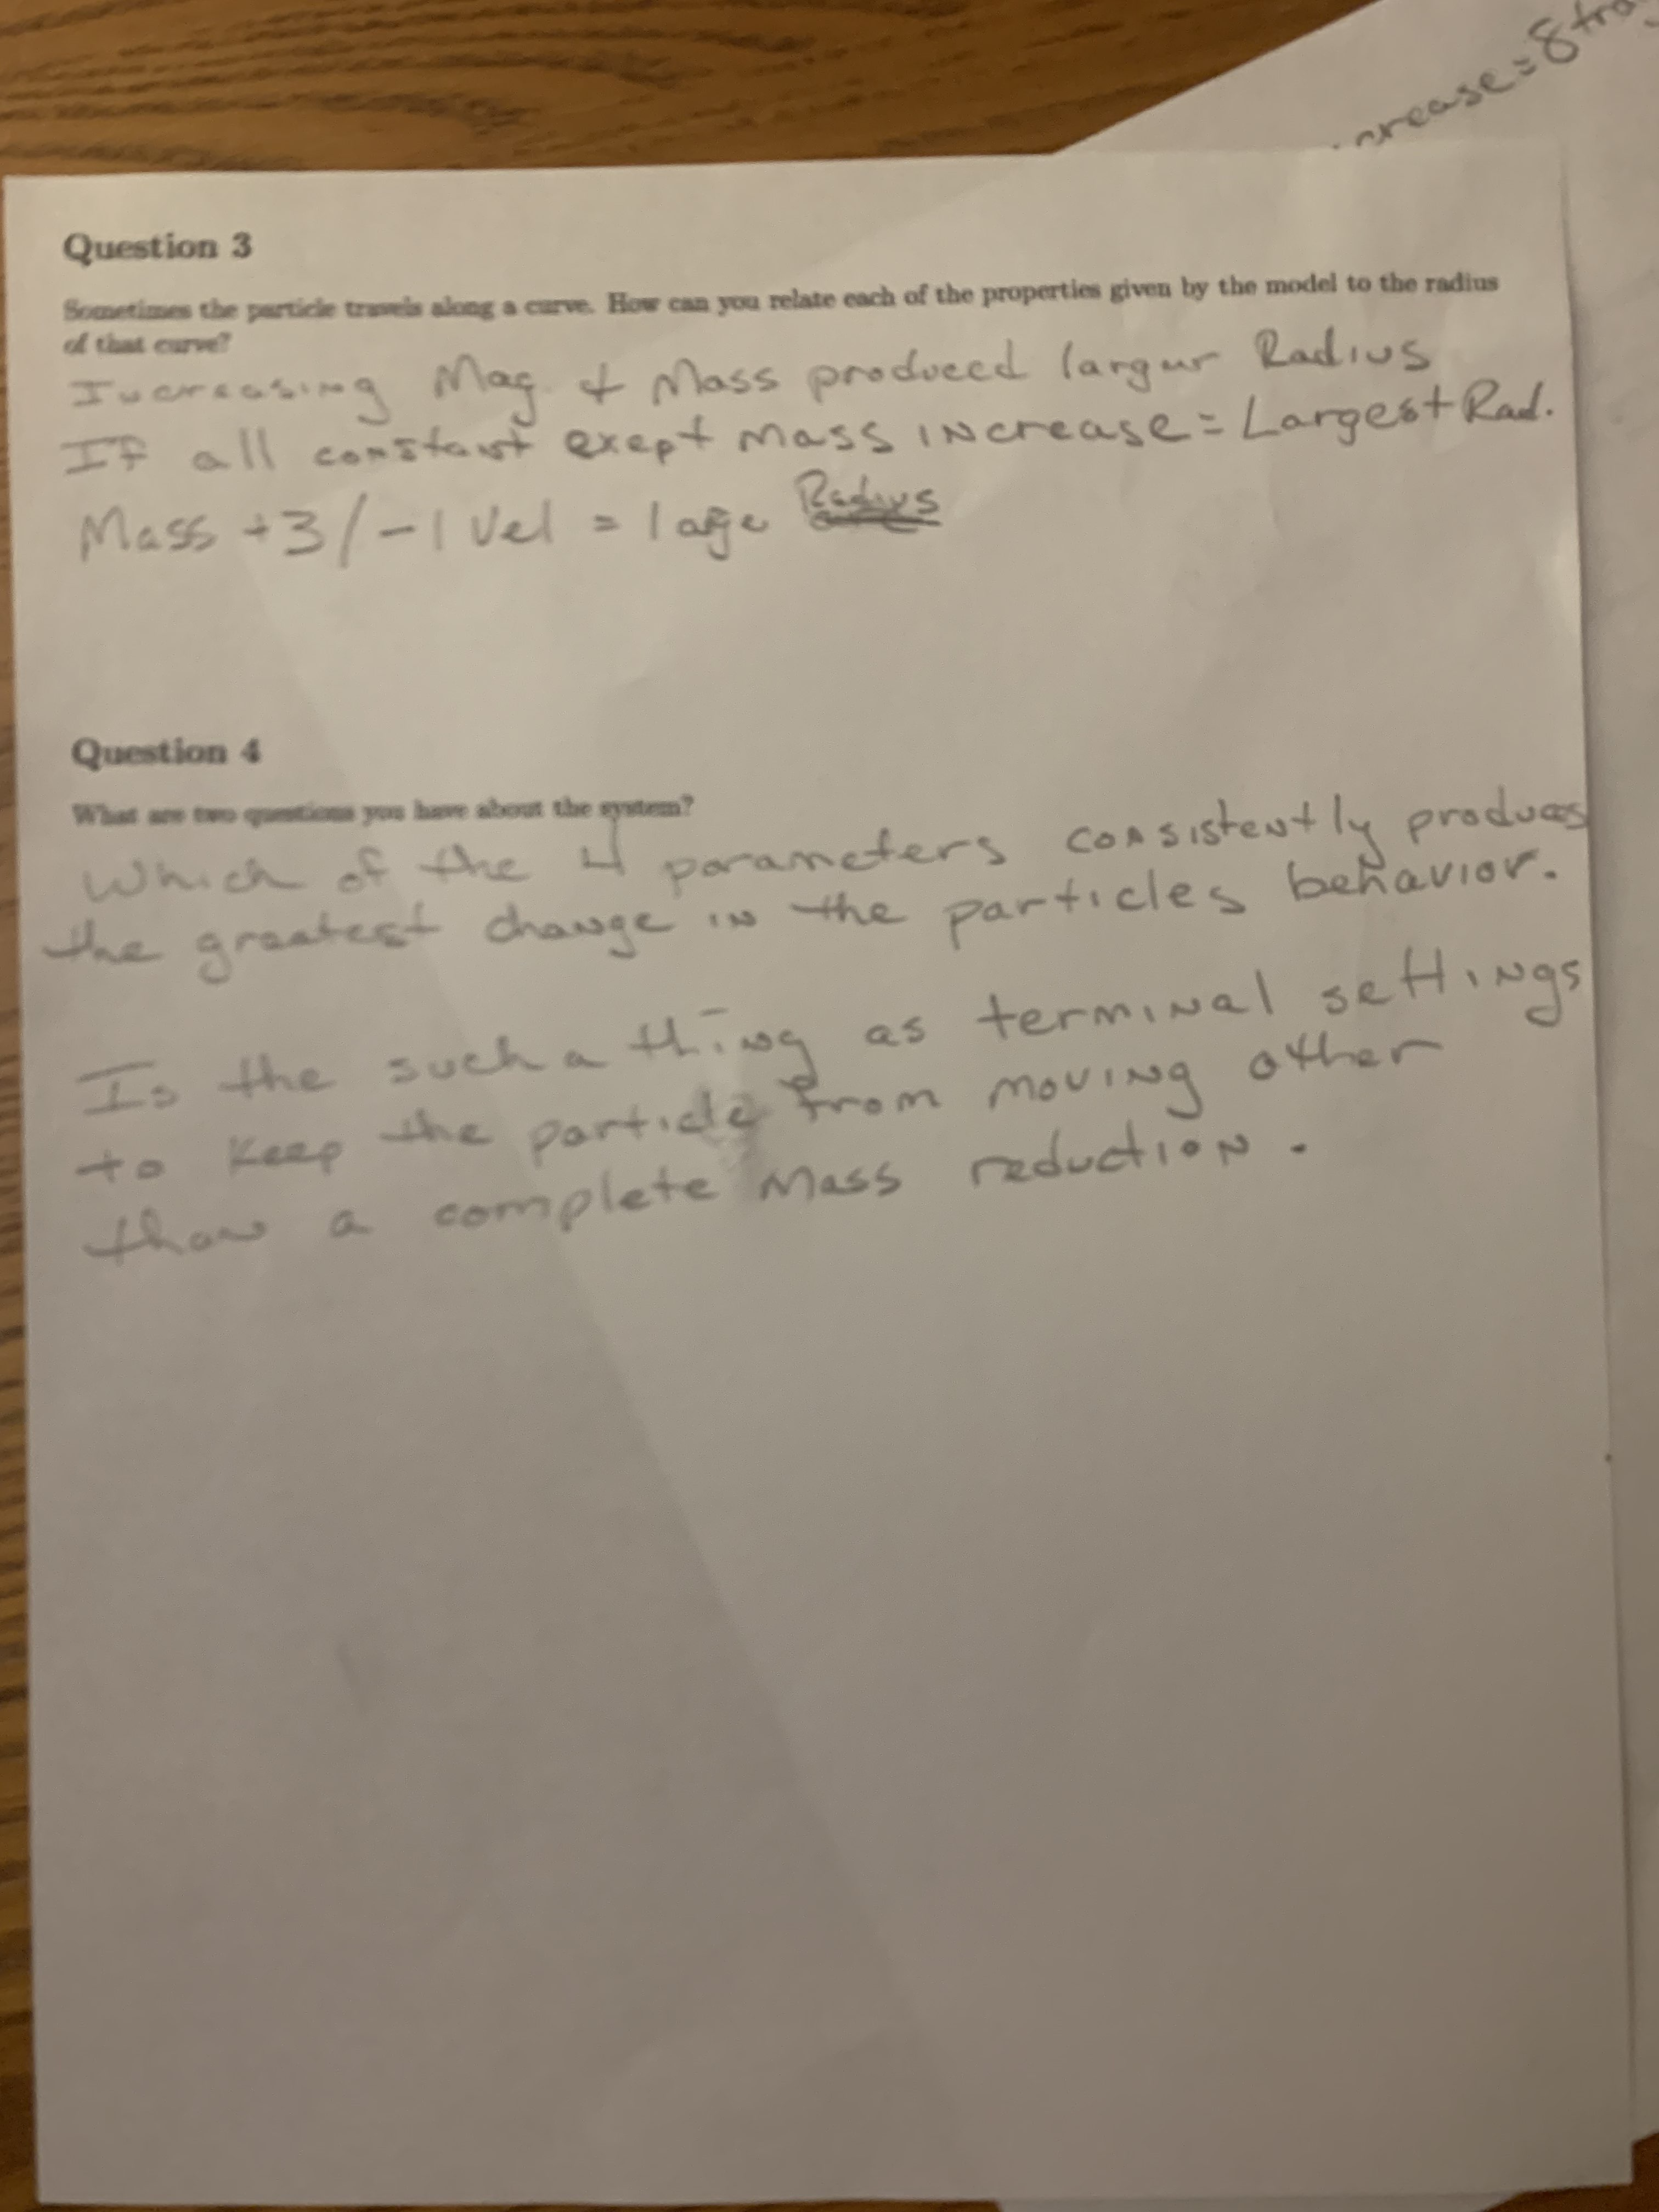
\includegraphics[scale = 0.15]{IMG_3}
		
		\section*{Analysis}
		
			Generally, I noticed a few unclear aspects of my model, some of which I have since corrected (The uncorrected model is in the supplemental files, if you want to see the differences firsthand). Scientific notation was intimidating for the subject, and so they tended to avoid utilizing the numbers. It also wasn't immediately clear what purpose the buttons that increase or decrease the parameters served, so making that connection clearer would be helpful. It also wasn't clear that the values for the initial parameters reset after each run, leading to some confusion on what caused circular motion. The subject also never made the connection between the vectors pointing into/out of the page during the simulation despite the direct explanation in the activity, which suggests that adding a more organic introduction for what the field represents would be helpful.
			
			It's interesting to note in question one that the subject primarily focused on superficial aspects of the model. I do think this still had a purpose, as it seemed to me during observation that this forced the subject to more closely examine aspects of the model.
			
			In question 2, the subject at first glance appears to have some incorrect statements. However, because they weren't looking at numerical values but instead at hitting the buttons, they wrote down that they decremented each of these values from the starting conditions. This means that they correctly identified that reducing the magnetic field or charge to 0 resulted in a straight line trajectory. They also self corrected an idea that mass impacted the trajectory, after observing a number of times where the mass was 3 AU and curved.
			
			In question 3, they identified some but not all of parameters that effected the radius of the particle's circular motion. Of note is the lack of experimentation with negative q and B values, which indicates that a question addressing that might help with understanding.
			
			In question 4, we can see some of their biggest questions. Of note is the idea that some factors might impact the radius more than others, where with a more numeric approach one could conceivably identify that they all have similar effects on magnitude. While the second question is a bit more confusing to read, it is interesting to note the emphasis on limiting behaviour, which is often seen by practicing physicists
			
			Generally, in terms of numeric understanding it's clear that not everything about the system was understood by the subject. Perhaps a more guided activity or more time would have helped with developing a clearer model. Another thing to note is that this isn't someone familiar with most physics concepts, so perhaps an intro physics student would be more likely to build a stronger model.
			
			There were pretty drastic results that I observed for engagement and general scientific thinking. The subject originally had a lot of trepidation for how much they could actually understand out of the model, and were initially very overwhelmed. However, they remained actively engaged with the activity throughout, with some notable "hmm"s and "huh"s as they corrected their conceptual understanding. Additionally, after the activity they noted that it was fun and felt that they took something away from it. It is possible and likely that there was bias due to the direct relation between myself and the subject, but as an observation it still shows promise for the power of engagement with models. Additionally, the model enhanced their scientific thinking by encouraging them to develop a model and correct it as new evidence arose. They started the activity trying random configurations, but slowly started systematically testing their model in different configurations in order to determine how the particle was behaving. This shows a lot of promise compared to more passive pre-class activities, as generally student alignment with expert views on scientific activities worsens in introductory classes.
			
			
			
			
			
\end{document}
